%%%%%%%%%%%%%%%%%%%%%%%%%%%%%%%%%%%%%%%%%%%%%%%%%%%%%%%%%%%%
% 1.5 RING THEORY
% The Composition of Advanced Mathematics
%%%%%%%%%%%%%%%%%%%%%%%%%%%%%%%%%%%%%%%%%%%%%%%%%%%%%%%%%%%%

\section{Ring Theory}
\label{sec:ring-theory}

\prerequisite{
Elementary set theory from \cref{sec:elementary-set-theory}, functions from
\cref{sec:functions}, elementary algebra from \cref{sec:elementary-algebra},
abstract algebra from \cref{sec:abstract-algebra}, and group theory from
\cref{sec:group-theory}.
}

\learningobjectives{
By the end of this section, the reader should be able to:
\begin{itemize}
    \item explain how rings extend the algebraic structure of groups;
    \item verify the ring axioms for common examples;
    \item distinguish commutative and noncommutative rings;
    \item identify zero divisors, units, nilpotent elements, and idempotents;
    \item work with subrings;
    \item understand integral domains and division rings;
    \item work with polynomial and matrix rings;
    \item recognize ideals and explain why they replace normal subgroups in ring theory;
    \item distinguish principal, prime, and maximal ideals at an introductory level;
    \item construct quotient rings;
    \item work with ring homomorphisms, kernels, and images;
    \item apply the First Isomorphism Theorem for rings;
    \item understand characteristic;
    \item recognize the structural relationship among rings, integral domains, division rings, and fields.
\end{itemize}
}

%%%%%%%%%%%%%%%%%%%%%%%%%%%%%%%%%%%%%%%%%%%%%%%%%%%%%%%%%%%%
\subsection{Why Rings?}
\label{subsec:why-rings}
%%%%%%%%%%%%%%%%%%%%%%%%%%%%%%%%%%%%%%%%%%%%%%%%%%%%%%%%%%%%

Groups study one reversible associative operation.

Many familiar mathematical systems, however, have two interacting operations.

The integers have both addition and multiplication:

\[ a+b,\qquad ab. \]

Polynomials can be added and multiplied.

Matrices can be added and multiplied.

Functions can be added and multiplied pointwise.

Modular arithmetic supports addition and multiplication.

Ring theory provides a common language for these systems.

\begin{conceptbox}
A ring is an algebraic structure equipped with two compatible operations,
usually called addition and multiplication.

Addition provides an abelian group structure, while multiplication interacts
with addition through the distributive laws.
\end{conceptbox}

%%%%%%%%%%%%%%%%%%%%%%%%%%%%%%%%%%%%%%%%%%%%%%%%%%%%%%%%%%%%
\subsection{From Groups to Rings}
\label{subsec:groups-to-rings}
%%%%%%%%%%%%%%%%%%%%%%%%%%%%%%%%%%%%%%%%%%%%%%%%%%%%%%%%%%%%

The structural transition can be pictured as

\begin{center}
\begin{tikzpicture}[
    node distance=18mm,
    box/.style={draw,rounded corners,align=center,inner sep=6pt},
    >=stealth
]
\node[box] (set) {Set};
\node[box,right=of set] (group) {Group\\one operation};
\node[box,right=of group] (ring) {Ring\\two operations};

\draw[->,thick] (set)--node[above]{add structure}(group);
\draw[->,thick] (group)--node[above]{add multiplication}(ring);
\end{tikzpicture}
\end{center}

The second operation cannot be arbitrary.

It must interact correctly with the additive structure.

%%%%%%%%%%%%%%%%%%%%%%%%%%%%%%%%%%%%%%%%%%%%%%%%%%%%%%%%%%%%
\subsection{Definition of a Ring}
\label{subsec:definition-ring}
%%%%%%%%%%%%%%%%%%%%%%%%%%%%%%%%%%%%%%%%%%%%%%%%%%%%%%%%%%%%

\begin{definitionbox}{Ring}
A \emph{ring} is a set \(R\) equipped with two binary operations, called
addition and multiplication, such that:

\begin{enumerate}
    \item \((R,+)\) is an abelian group;
    \item multiplication is associative:
    \[ (ab)c=a(bc); \]
    \item multiplication distributes over addition:
    \[ a(b+c)=ab+ac, \]
    \[ (a+b)c=ac+bc. \]
\end{enumerate}
\end{definitionbox}

Throughout this text, unless explicitly stated otherwise, a ring is assumed to
have a multiplicative identity \(1\).

This convention is important because different algebra texts use slightly
different definitions of a ring.

%%%%%%%%%%%%%%%%%%%%%%%%%%%%%%%%%%%%%%%%%%%%%%%%%%%%%%%%%%%%
\subsection{The Two Operations}
\label{subsec:ring-two-operations}
%%%%%%%%%%%%%%%%%%%%%%%%%%%%%%%%%%%%%%%%%%%%%%%%%%%%%%%%%%%%

A ring has two operations with different structural roles.

Addition gives:

\begin{itemize}
    \item closure;
    \item associativity;
    \item additive identity \(0\);
    \item additive inverses;
    \item commutativity.
\end{itemize}

Multiplication gives:

\begin{itemize}
    \item closure;
    \item associativity;
    \item multiplicative identity \(1\) under our convention.
\end{itemize}

Multiplication need not be commutative.

The distributive laws connect the two operations.

%%%%%%%%%%%%%%%%%%%%%%%%%%%%%%%%%%%%%%%%%%%%%%%%%%%%%%%%%%%%
\subsection{Visual Structure of a Ring}
\label{subsec:visual-ring-structure}
%%%%%%%%%%%%%%%%%%%%%%%%%%%%%%%%%%%%%%%%%%%%%%%%%%%%%%%%%%%%

\begin{center}
\begin{tikzpicture}[
    node distance=13mm and 22mm,
    box/.style={draw,rounded corners,align=center,inner sep=5pt},
    >=stealth
]
\node[box] (R) {Ring \(R\)};
\node[box,below left=of R] (add) {Addition\\abelian group};
\node[box,below right=of R] (mult) {Multiplication\\associative};
\node[box,below=18mm of R] (dist) {Distributive laws};

\draw[->] (R)--(add);
\draw[->] (R)--(mult);
\draw[->] (add)--(dist);
\draw[->] (mult)--(dist);
\end{tikzpicture}
\end{center}

The distributive laws are the bridge between the additive and multiplicative
structures.

%%%%%%%%%%%%%%%%%%%%%%%%%%%%%%%%%%%%%%%%%%%%%%%%%%%%%%%%%%%%
\subsection{The Integers}
\label{subsec:integers-ring-theory}
%%%%%%%%%%%%%%%%%%%%%%%%%%%%%%%%%%%%%%%%%%%%%%%%%%%%%%%%%%%%

The standard example of a ring is

\[ \Z. \]

Under ordinary addition,

\[ (\Z,+) \]

is an abelian group.

Integer multiplication is associative and has identity \(1\).

The distributive laws hold.

Therefore,

\[ (\Z,+,\cdot) \]

is a ring.

%%%%%%%%%%%%%%%%%%%%%%%%%%%%%%%%%%%%%%%%%%%%%%%%%%%%%%%%%%%%
\subsection{Other Familiar Rings}
\label{subsec:familiar-rings}
%%%%%%%%%%%%%%%%%%%%%%%%%%%%%%%%%%%%%%%%%%%%%%%%%%%%%%%%%%%%

Other examples include

\[ \Q,\qquad \R,\qquad \C. \]

These are more than rings: they are fields.

The modular integers

\[ \Z_n \]

also form rings under addition and multiplication modulo \(n\).

Polynomial sets such as

\[ \R[x] \]

form rings.

Square matrices

\[ M_n(\R) \]

form rings.

%%%%%%%%%%%%%%%%%%%%%%%%%%%%%%%%%%%%%%%%%%%%%%%%%%%%%%%%%%%%
\subsection{Commutative Rings}
\label{subsec:commutative-rings}
%%%%%%%%%%%%%%%%%%%%%%%%%%%%%%%%%%%%%%%%%%%%%%%%%%%%%%%%%%%%

\begin{definitionbox}{Commutative Ring}
A ring \(R\) is \emph{commutative} if
\[ ab=ba \]
for every \(a,b\in R\).
\end{definitionbox}

The rings

\[ \Z,\qquad\Q,\qquad\R,\qquad\C \]

are commutative.

Matrix rings generally are not.

%%%%%%%%%%%%%%%%%%%%%%%%%%%%%%%%%%%%%%%%%%%%%%%%%%%%%%%%%%%%
\subsection{Matrix Rings}
\label{subsec:matrix-rings}
%%%%%%%%%%%%%%%%%%%%%%%%%%%%%%%%%%%%%%%%%%%%%%%%%%%%%%%%%%%%

Let

\[ M_n(\R) \]

denote the set of all \(n\times n\) real matrices.

Matrix addition and multiplication make \(M_n(\R)\) a ring.

The additive identity is the zero matrix

\[ \zero. \]

The multiplicative identity is

\[ I_n. \]

However, matrix multiplication is generally noncommutative.

%%%%%%%%%%%%%%%%%%%%%%%%%%%%%%%%%%%%%%%%%%%%%%%%%%%%%%%%%%%%
\subsection{A Visual Example of Noncommutativity}
\label{subsec:ring-noncommutative-visual}
%%%%%%%%%%%%%%%%%%%%%%%%%%%%%%%%%%%%%%%%%%%%%%%%%%%%%%%%%%%%

Consider

\[ A=\begin{pmatrix}1&1\\0&1\end{pmatrix},\qquad B=\begin{pmatrix}1&0\\1&1\end{pmatrix}. \]

Then

\[ AB=\begin{pmatrix}2&1\\1&1\end{pmatrix},\qquad BA=\begin{pmatrix}1&1\\1&2\end{pmatrix}. \]

Therefore,

\[ AB\neq BA. \]

The difference can be visualized structurally as

\begin{center}
\begin{tikzpicture}[
    node distance=16mm,
    box/.style={draw,rounded corners,align=center,minimum width=18mm,minimum height=9mm},
    >=stealth
]
\node[box] (v1) {\(\vect{x}\)};
\node[box,right=of v1] (b1) {\(B\vect{x}\)};
\node[box,right=of b1] (ab) {\(AB\vect{x}\)};

\node[box,below=of v1] (v2) {\(\vect{x}\)};
\node[box,right=of v2] (a1) {\(A\vect{x}\)};
\node[box,right=of a1] (ba) {\(BA\vect{x}\)};

\draw[->,thick] (v1)--node[above]{\(B\)}(b1);
\draw[->,thick] (b1)--node[above]{\(A\)}(ab);
\draw[->,thick] (v2)--node[above]{\(A\)}(a1);
\draw[->,thick] (a1)--node[above]{\(B\)}(ba);

\node[right=8mm of ab] {\(\neq\)};
\node[right=8mm of ba] {};
\end{tikzpicture}
\end{center}

Applying \(B\) then \(A\) need not give the same transformation as applying
\(A\) then \(B\).

%%%%%%%%%%%%%%%%%%%%%%%%%%%%%%%%%%%%%%%%%%%%%%%%%%%%%%%%%%%%
\subsection{Basic Ring Identities}
\label{subsec:basic-ring-identities}
%%%%%%%%%%%%%%%%%%%%%%%%%%%%%%%%%%%%%%%%%%%%%%%%%%%%%%%%%%%%

Many familiar arithmetic rules follow from the ring axioms.

\begin{theorem}
For every \(a\in R\),
\[ a0=0a=0. \]
\end{theorem}

\begin{proof}
Since

\[ 0+0=0, \]

we have

\[ a0=a(0+0)=a0+a0. \]

Add \(-(a0)\) to both sides:

\[ 0=a0. \]

Similarly,

\[ 0a=0. \]
\end{proof}

%%%%%%%%%%%%%%%%%%%%%%%%%%%%%%%%%%%%%%%%%%%%%%%%%%%%%%%%%%%%
\subsection{Negative Elements and Multiplication}
\label{subsec:ring-negative-elements}
%%%%%%%%%%%%%%%%%%%%%%%%%%%%%%%%%%%%%%%%%%%%%%%%%%%%%%%%%%%%

\begin{theorem}
For all \(a,b\in R\),
\[ (-a)b=-(ab),\qquad a(-b)=-(ab). \]
\end{theorem}

Consequently,

\[ (-a)(-b)=ab. \]

Thus familiar sign rules are consequences of ring structure rather than
independent arithmetic facts.

%%%%%%%%%%%%%%%%%%%%%%%%%%%%%%%%%%%%%%%%%%%%%%%%%%%%%%%%%%%%
\subsection{The Binomial Formula and Commutativity}
\label{subsec:ring-binomial-formula}
%%%%%%%%%%%%%%%%%%%%%%%%%%%%%%%%%%%%%%%%%%%%%%%%%%%%%%%%%%%%

In a commutative ring,

\[ (a+b)^2=a^2+2ab+b^2. \]

But in a noncommutative ring,

\[ (a+b)^2=a^2+ab+ba+b^2. \]

Since \(ab\) and \(ba\) may differ, they cannot necessarily be combined into

\[ 2ab. \]

\begin{warningbox}
Many elementary algebra identities silently depend on commutativity.

When working in an arbitrary ring, always determine whether factors may be
reordered.
\end{warningbox}

%%%%%%%%%%%%%%%%%%%%%%%%%%%%%%%%%%%%%%%%%%%%%%%%%%%%%%%%%%%%
\subsection{Zero Divisors}
\label{subsec:zero-divisors}
%%%%%%%%%%%%%%%%%%%%%%%%%%%%%%%%%%%%%%%%%%%%%%%%%%%%%%%%%%%%

In ordinary real-number arithmetic,

\[ ab=0 \]

implies

\[ a=0\qquad\text{or}\qquad b=0. \]

This property does not hold in every ring.

\begin{definitionbox}{Zero Divisor}
A nonzero element \(a\in R\) is a \emph{zero divisor} if there exists a
nonzero \(b\in R\) such that
\[ ab=0 \]
or
\[ ba=0. \]
\end{definitionbox}

%%%%%%%%%%%%%%%%%%%%%%%%%%%%%%%%%%%%%%%%%%%%%%%%%%%%%%%%%%%%
\subsection{Example of Zero Divisors}
\label{subsec:zero-divisor-example}
%%%%%%%%%%%%%%%%%%%%%%%%%%%%%%%%%%%%%%%%%%%%%%%%%%%%%%%%%%%%

Consider \(\Z_6\).

We have

\[ [2]_6[3]_6=[6]_6=[0]_6. \]

Yet

\[ [2]_6\neq[0]_6,\qquad[3]_6\neq[0]_6. \]

Therefore \([2]_6\) and \([3]_6\) are zero divisors.

%%%%%%%%%%%%%%%%%%%%%%%%%%%%%%%%%%%%%%%%%%%%%%%%%%%%%%%%%%%%
\subsection{Visualizing Zero Divisors in Modular Arithmetic}
\label{subsec:visual-zero-divisors}
%%%%%%%%%%%%%%%%%%%%%%%%%%%%%%%%%%%%%%%%%%%%%%%%%%%%%%%%%%%%

\begin{center}
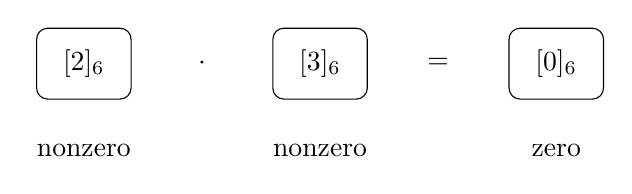
\begin{tikzpicture}[
    box/.style={draw,rounded corners,minimum width=12mm,minimum height=9mm},
    >=stealth
]
\node[box] (a) at (0,0) {\([2]_6\)};
\node at (1.5,0) {\(\cdot\)};
\node[box] (b) at (3,0) {\([3]_6\)};
\node at (4.5,0) {\(=\)};
\node[box] (z) at (6,0) {\([0]_6\)};

\node at (0,-1.1) {nonzero};
\node at (3,-1.1) {nonzero};
\node at (6,-1.1) {zero};
\end{tikzpicture}
\end{center}

This behavior is impossible in an integral domain.

%%%%%%%%%%%%%%%%%%%%%%%%%%%%%%%%%%%%%%%%%%%%%%%%%%%%%%%%%%%%
\subsection{Cancellation and Zero Divisors}
\label{subsec:ring-cancellation-zero-divisors}
%%%%%%%%%%%%%%%%%%%%%%%%%%%%%%%%%%%%%%%%%%%%%%%%%%%%%%%%%%%%

Suppose

\[ ab=ac. \]

Then

\[ ab-ac=0. \]

By distributivity,

\[ a(b-c)=0. \]

If \(a\neq0\) and the ring has no zero divisors, then

\[ b-c=0, \]

so

\[ b=c. \]

Thus the absence of zero divisors allows multiplicative cancellation of
nonzero elements.

%%%%%%%%%%%%%%%%%%%%%%%%%%%%%%%%%%%%%%%%%%%%%%%%%%%%%%%%%%%%
\subsection{Units}
\label{subsec:ring-units}
%%%%%%%%%%%%%%%%%%%%%%%%%%%%%%%%%%%%%%%%%%%%%%%%%%%%%%%%%%%%

\begin{definitionbox}{Unit}
An element \(u\in R\) is a \emph{unit} if it has a multiplicative inverse in
\(R\).

That is, there exists \(v\in R\) such that
\[ uv=vu=1. \]
\end{definitionbox}

The element \(v\) is written

\[ u^{-1}. \]

The units of a ring form a group under multiplication.

This group is often denoted

\[ R^\times. \]

The notation \(R^\times\) is read ``R cross'' or ``the group of units of
\(R\).''

%%%%%%%%%%%%%%%%%%%%%%%%%%%%%%%%%%%%%%%%%%%%%%%%%%%%%%%%%%%%
\subsection{Units in the Integers}
\label{subsec:integer-units}
%%%%%%%%%%%%%%%%%%%%%%%%%%%%%%%%%%%%%%%%%%%%%%%%%%%%%%%%%%%%

In \(\Z\), the only units are

\[ 1\qquad\text{and}\qquad -1. \]

Indeed,

\[ 1^{-1}=1,\qquad(-1)^{-1}=-1. \]

No other integer has a multiplicative inverse that is also an integer.

Therefore,

\[ \Z^\times=\{-1,1\}. \]

%%%%%%%%%%%%%%%%%%%%%%%%%%%%%%%%%%%%%%%%%%%%%%%%%%%%%%%%%%%%
\subsection{Units Modulo \(n\)}
\label{subsec:units-mod-n}
%%%%%%%%%%%%%%%%%%%%%%%%%%%%%%%%%%%%%%%%%%%%%%%%%%%%%%%%%%%%

In \(\Z_n\), the class \([a]_n\) is a unit precisely when

\[ \gcd(a,n)=1. \]

The notation

\[ \gcd(a,n) \]

means the \emph{greatest common divisor} of \(a\) and \(n\), and is read
``the greatest common divisor of \(a\) and \(n\).''

For example, in \(\Z_8\),

\[ [1]_8,\ [3]_8,\ [5]_8,\ [7]_8 \]

are units.

%%%%%%%%%%%%%%%%%%%%%%%%%%%%%%%%%%%%%%%%%%%%%%%%%%%%%%%%%%%%
\subsection{Worked Example: Units in \(\Z_{10}\)}
\label{subsec:worked-units-z10}
%%%%%%%%%%%%%%%%%%%%%%%%%%%%%%%%%%%%%%%%%%%%%%%%%%%%%%%%%%%%

\begin{workedexamplebox}{Finding Units Modulo \(10\)}

Determine the units of \(\Z_{10}\).

\begin{tabularx}{\textwidth}{@{}>{\raggedright\arraybackslash}p{0.42\textwidth}X@{}}
A class is a unit when its representative is relatively prime to \(10\). & \(\gcd(a,10)=1\)\\
Check representatives \(0,\ldots,9\). & \(1,3,7,9\) are relatively prime to \(10\).\\
Write the unit group. & \(\Z_{10}^{\times}=\{[1],[3],[7],[9]\}\)
\end{tabularx}

\begin{answerbox}
\[ \Z_{10}^{\times}=\{[1]_{10},[3]_{10},[7]_{10},[9]_{10}\}. \]
\end{answerbox}
\end{workedexamplebox}

%%%%%%%%%%%%%%%%%%%%%%%%%%%%%%%%%%%%%%%%%%%%%%%%%%%%%%%%%%%%
\subsection{Nilpotent Elements}
\label{subsec:nilpotent-elements}
%%%%%%%%%%%%%%%%%%%%%%%%%%%%%%%%%%%%%%%%%%%%%%%%%%%%%%%%%%%%

\begin{definitionbox}{Nilpotent Element}
An element \(a\in R\) is \emph{nilpotent} if
\[ a^n=0 \]
for some positive integer \(n\).
\end{definitionbox}

For example, in \(\Z_4\),

\[ [2]_4^2=[4]_4=[0]_4. \]

Therefore \([2]_4\) is nilpotent.

%%%%%%%%%%%%%%%%%%%%%%%%%%%%%%%%%%%%%%%%%%%%%%%%%%%%%%%%%%%%
\subsection{Idempotent Elements}
\label{subsec:idempotent-elements}
%%%%%%%%%%%%%%%%%%%%%%%%%%%%%%%%%%%%%%%%%%%%%%%%%%%%%%%%%%%%

\begin{definitionbox}{Idempotent Element}
An element \(a\in R\) is \emph{idempotent} if
\[ a^2=a. \]
\end{definitionbox}

The elements \(0\) and \(1\) are always idempotent.

Some rings contain additional idempotents.

For example, in \(\Z_6\),

\[ [3]_6^2=[9]_6=[3]_6. \]

Thus \([3]_6\) is idempotent.

%%%%%%%%%%%%%%%%%%%%%%%%%%%%%%%%%%%%%%%%%%%%%%%%%%%%%%%%%%%%
\subsection{Subrings}
\label{subsec:subrings}
%%%%%%%%%%%%%%%%%%%%%%%%%%%%%%%%%%%%%%%%%%%%%%%%%%%%%%%%%%%%

\begin{definitionbox}{Subring}
A subset \(S\subseteq R\) is a \emph{subring} if it forms a ring under the
operations inherited from \(R\).
\end{definitionbox}

Under the convention that rings contain \(1\), we generally require a subring
to contain the same multiplicative identity unless explicitly stated
otherwise.

For example,

\[ \Z\subseteq\Q\subseteq\R\subseteq\C. \]

Each inclusion gives a familiar ring sitting inside a larger ring.

%%%%%%%%%%%%%%%%%%%%%%%%%%%%%%%%%%%%%%%%%%%%%%%%%%%%%%%%%%%%
\subsection{Subring Test}
\label{subsec:subring-test}
%%%%%%%%%%%%%%%%%%%%%%%%%%%%%%%%%%%%%%%%%%%%%%%%%%%%%%%%%%%%

A useful test is the following.

\begin{theorem}[Subring Test]
Let \(S\) be a nonempty subset of a ring \(R\). If for every \(a,b\in S\),

\[ a-b\in S \]

and

\[ ab\in S, \]

then \(S\) is closed under the additive group structure and multiplication.

Under the unital convention, also verify that the required identity belongs
to \(S\).
\end{theorem}

%%%%%%%%%%%%%%%%%%%%%%%%%%%%%%%%%%%%%%%%%%%%%%%%%%%%%%%%%%%%
\subsection{Integral Domains}
\label{subsec:integral-domains}
%%%%%%%%%%%%%%%%%%%%%%%%%%%%%%%%%%%%%%%%%%%%%%%%%%%%%%%%%%%%

\begin{definitionbox}{Integral Domain}
An \emph{integral domain} is a commutative ring with identity
\[ 1\neq0 \]
and no zero divisors.
\end{definitionbox}

The integers \(\Z\) form an integral domain.

The ring \(\Z_6\) does not because

\[ [2]_6[3]_6=[0]_6. \]

%%%%%%%%%%%%%%%%%%%%%%%%%%%%%%%%%%%%%%%%%%%%%%%%%%%%%%%%%%%%
\subsection{Why Integral Domains Matter}
\label{subsec:why-integral-domains}
%%%%%%%%%%%%%%%%%%%%%%%%%%%%%%%%%%%%%%%%%%%%%%%%%%%%%%%%%%%%

Integral domains preserve several important features of ordinary arithmetic.

For nonzero \(a\),

\[ ab=ac\Longrightarrow b=c. \]

Also,

\[ ab=0\Longrightarrow a=0\text{ or }b=0. \]

These properties make integral domains behave much more like the integers
than arbitrary rings do.

%%%%%%%%%%%%%%%%%%%%%%%%%%%%%%%%%%%%%%%%%%%%%%%%%%%%%%%%%%%%
\subsection{Division Rings}
\label{subsec:division-rings}
%%%%%%%%%%%%%%%%%%%%%%%%%%%%%%%%%%%%%%%%%%%%%%%%%%%%%%%%%%%%

\begin{definitionbox}{Division Ring}
A \emph{division ring} is a ring in which every nonzero element is a unit.
\end{definitionbox}

Multiplication need not be commutative.

Thus division rings generalize fields by allowing noncommutative
multiplication.

A famous example is the ring of quaternions.

%%%%%%%%%%%%%%%%%%%%%%%%%%%%%%%%%%%%%%%%%%%%%%%%%%%%%%%%%%%%
\subsection{The Quaternions}
\label{subsec:quaternions-ring}
%%%%%%%%%%%%%%%%%%%%%%%%%%%%%%%%%%%%%%%%%%%%%%%%%%%%%%%%%%%%

The quaternions are written

\[ \mathbb{H}=\{a+bi+cj+dk:a,b,c,d\in\R\}. \]

The symbol

\[ \mathbb{H} \]

is commonly used for the quaternions and is read ``blackboard-bold H'' or
simply ``the quaternions.''

Their fundamental multiplication rules include

\[ i^2=j^2=k^2=-1 \]

and

\[ ij=k,\qquad jk=i,\qquad ki=j. \]

Reversing the order changes signs:

\[ ji=-k,\qquad kj=-i,\qquad ik=-j. \]

Thus quaternion multiplication is noncommutative.

%%%%%%%%%%%%%%%%%%%%%%%%%%%%%%%%%%%%%%%%%%%%%%%%%%%%%%%%%%%%
\subsection{Visualizing the Number-System Extension}
\label{subsec:number-system-ring-extension}
%%%%%%%%%%%%%%%%%%%%%%%%%%%%%%%%%%%%%%%%%%%%%%%%%%%%%%%%%%%%

\begin{center}
\begin{tikzpicture}[
    node distance=13mm,
    box/.style={draw,rounded corners,minimum width=13mm,minimum height=8mm},
    >=stealth
]
\node[box] (Z) {\(\Z\)};
\node[box,right=of Z] (Q) {\(\Q\)};
\node[box,right=of Q] (R) {\(\R\)};
\node[box,right=of R] (C) {\(\C\)};
\node[box,right=of C] (H) {\(\mathbb H\)};

\draw[->,thick] (Z)--(Q);
\draw[->,thick] (Q)--(R);
\draw[->,thick] (R)--(C);
\draw[->,thick] (C)--(H);

\node[below=4mm of Z] {\small domain};
\node[below=4mm of Q] {\small field};
\node[below=4mm of R] {\small field};
\node[below=4mm of C] {\small field};
\node[below=4mm of H] {\small division ring};
\end{tikzpicture}
\end{center}

The final step sacrifices commutative multiplication.

%%%%%%%%%%%%%%%%%%%%%%%%%%%%%%%%%%%%%%%%%%%%%%%%%%%%%%%%%%%%
\subsection{Fields in the Ring Hierarchy}
\label{subsec:fields-ring-hierarchy}
%%%%%%%%%%%%%%%%%%%%%%%%%%%%%%%%%%%%%%%%%%%%%%%%%%%%%%%%%%%%

A field is a commutative division ring.

Thus every nonzero element has a multiplicative inverse and multiplication is
commutative.

Examples are

\[ \Q,\qquad\R,\qquad\C. \]

Field theory is developed in detail in \cref{sec:field-theory}.

%%%%%%%%%%%%%%%%%%%%%%%%%%%%%%%%%%%%%%%%%%%%%%%%%%%%%%%%%%%%
\subsection{Hierarchy of Ring-Like Structures}
\label{subsec:ring-hierarchy}
%%%%%%%%%%%%%%%%%%%%%%%%%%%%%%%%%%%%%%%%%%%%%%%%%%%%%%%%%%%%

The relationships can be summarized visually.

\begin{center}
\begin{tikzpicture}[
    node distance=10mm,
    box/.style={draw,rounded corners,align=center,inner sep=5pt,font=\small},
    >=stealth
]
\node[box] (ring) {Ring};
\node[box,below=of ring] (comm) {Commutative ring};
\node[box,below=of comm] (domain) {Integral domain};
\node[box,below left=of domain] (field) {Field};

\node[box,right=30mm of domain] (division) {Division ring};

\draw[->] (ring)--(comm);
\draw[->] (comm)--(domain);
\draw[->] (domain)--(field);
\draw[->] (division)--(field);

\node[right=4mm of field] {\small commutative division ring};
\end{tikzpicture}
\end{center}

The arrows indicate the addition of stronger conditions, not that every ring
automatically belongs to the more restrictive classes.

%%%%%%%%%%%%%%%%%%%%%%%%%%%%%%%%%%%%%%%%%%%%%%%%%%%%%%%%%%%%
\subsection{Polynomial Rings}
\label{subsec:polynomial-rings}
%%%%%%%%%%%%%%%%%%%%%%%%%%%%%%%%%%%%%%%%%%%%%%%%%%%%%%%%%%%%

Let \(R\) be a commutative ring.

The polynomial ring over \(R\) is written

\[ R[x]. \]

Its elements have the form

\[ a_0+a_1x+a_2x^2+\cdots+a_nx^n, \]

where

\[ a_0,a_1,\ldots,a_n\in R. \]

The notation \(R[x]\) is read ``R adjoin \(x\)'' or ``the polynomial ring in
\(x\) over \(R\).''

%%%%%%%%%%%%%%%%%%%%%%%%%%%%%%%%%%%%%%%%%%%%%%%%%%%%%%%%%%%%
\subsection{Examples of Polynomial Rings}
\label{subsec:polynomial-ring-examples}
%%%%%%%%%%%%%%%%%%%%%%%%%%%%%%%%%%%%%%%%%%%%%%%%%%%%%%%%%%%%

Examples include

\[ \Z[x],\qquad\Q[x],\qquad\R[x],\qquad\C[x]. \]

A polynomial in \(\Z[x]\) might be

\[ 3x^4-2x+7. \]

A polynomial in \(\Z_5[x]\) has coefficients interpreted modulo \(5\).

%%%%%%%%%%%%%%%%%%%%%%%%%%%%%%%%%%%%%%%%%%%%%%%%%%%%%%%%%%%%
\subsection{Polynomial Arithmetic}
\label{subsec:ring-polynomial-arithmetic}
%%%%%%%%%%%%%%%%%%%%%%%%%%%%%%%%%%%%%%%%%%%%%%%%%%%%%%%%%%%%

Polynomial addition is performed coefficientwise.

For example,

\[ (x^2+2x+1)+(2x^2-x+3)=3x^2+x+4. \]

Polynomial multiplication uses distributivity.

\[ (x+1)(x+2)=x^2+3x+2. \]

The familiar polynomial rules are therefore manifestations of ring axioms.

%%%%%%%%%%%%%%%%%%%%%%%%%%%%%%%%%%%%%%%%%%%%%%%%%%%%%%%%%%%%
\subsection{Degree}
\label{subsec:ring-polynomial-degree}
%%%%%%%%%%%%%%%%%%%%%%%%%%%%%%%%%%%%%%%%%%%%%%%%%%%%%%%%%%%%

For a nonzero polynomial \(f(x)\), its degree is written

\[ \deg f. \]

The notation is read ``the degree of \(f\).''

For example,

\[ f(x)=7x^5-2x^2+1 \]

has

\[ \deg f=5. \]

If \(R\) is an integral domain and \(f,g\neq0\), then

\[ \deg(fg)=\deg f+\deg g. \]

This can fail over rings with zero divisors.

%%%%%%%%%%%%%%%%%%%%%%%%%%%%%%%%%%%%%%%%%%%%%%%%%%%%%%%%%%%%
\subsection{Why Zero Divisors Affect Polynomial Degree}
\label{subsec:zero-divisor-polynomial-degree}
%%%%%%%%%%%%%%%%%%%%%%%%%%%%%%%%%%%%%%%%%%%%%%%%%%%%%%%%%%%%

Consider \(\Z_6[x]\).

Let

\[ f(x)=2x+1,\qquad g(x)=3x+1. \]

Then

\[ f(x)g(x)=6x^2+5x+1. \]

Modulo \(6\),

\[ 6x^2=0. \]

Therefore,

\[ f(x)g(x)=5x+1. \]

Although both factors have degree \(1\), their product has degree \(1\), not
\(2\).

%%%%%%%%%%%%%%%%%%%%%%%%%%%%%%%%%%%%%%%%%%%%%%%%%%%%%%%%%%%%
\subsection{Ideals}
\label{subsec:ideals}
%%%%%%%%%%%%%%%%%%%%%%%%%%%%%%%%%%%%%%%%%%%%%%%%%%%%%%%%%%%%

Subrings describe smaller rings inside larger rings.

For quotient constructions, however, a stronger type of subset is needed.

\begin{definitionbox}{Ideal}
A subset \(I\subseteq R\) is an \emph{ideal} if:

\begin{enumerate}
    \item \(I\) is an additive subgroup of \(R\);
    \item for every \(r\in R\) and \(a\in I\),
    \[ ra\in I,\qquad ar\in I. \]
\end{enumerate}
\end{definitionbox}

The notation

\[ I\trianglelefteq R \]

may be used to indicate that \(I\) is an ideal of \(R\).

%%%%%%%%%%%%%%%%%%%%%%%%%%%%%%%%%%%%%%%%%%%%%%%%%%%%%%%%%%%%
\subsection{Visualizing an Ideal}
\label{subsec:visual-ideal}
%%%%%%%%%%%%%%%%%%%%%%%%%%%%%%%%%%%%%%%%%%%%%%%%%%%%%%%%%%%%

\begin{center}
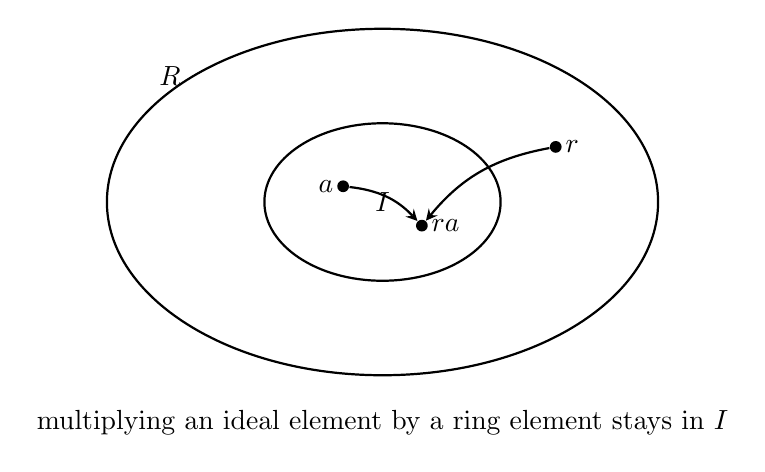
\begin{tikzpicture}[>=stealth]
\draw[thick] (0,0) ellipse (3.5 and 2.2);
\draw[thick] (0,0) ellipse (1.5 and 1);

\node at (-2.7,1.6) {\(R\)};
\node at (0,0) {\(I\)};

\node[circle,fill,inner sep=1.5pt] (r) at (2.2,0.7) {};
\node[circle,fill,inner sep=1.5pt] (a) at (-0.5,0.2) {};
\node[circle,fill,inner sep=1.5pt] (ra) at (0.5,-0.3) {};

\node[right] at (r) {\(r\)};
\node[left] at (a) {\(a\)};
\node[right] at (ra) {\(ra\)};

\draw[->,thick] (r) to[bend right=20] (ra);
\draw[->,thick] (a) to[bend left=20] (ra);

\node at (0,-2.8) {multiplying an ideal element by a ring element stays in \(I\)};
\end{tikzpicture}
\end{center}

An ideal absorbs multiplication by elements of the surrounding ring.

%%%%%%%%%%%%%%%%%%%%%%%%%%%%%%%%%%%%%%%%%%%%%%%%%%%%%%%%%%%%
\subsection{Ideals and Normal Subgroups}
\label{subsec:ideals-normal-subgroups}
%%%%%%%%%%%%%%%%%%%%%%%%%%%%%%%%%%%%%%%%%%%%%%%%%%%%%%%%%%%%

There is a useful analogy:

\[
\begin{array}{c|c}
\text{Group theory} & \text{Ring theory}\\
\hline
\text{subgroup} & \text{subring}\\
\text{normal subgroup} & \text{ideal}\\
\text{quotient group} & \text{quotient ring}\\
\text{group homomorphism kernel} & \text{ring homomorphism kernel}
\end{array}
\]

Normal subgroups are exactly the subgroup structures needed to form quotient
groups.

Ideals play the corresponding role for rings.

%%%%%%%%%%%%%%%%%%%%%%%%%%%%%%%%%%%%%%%%%%%%%%%%%%%%%%%%%%%%
\subsection{Principal Ideals}
\label{subsec:principal-ideals}
%%%%%%%%%%%%%%%%%%%%%%%%%%%%%%%%%%%%%%%%%%%%%%%%%%%%%%%%%%%%

\begin{definitionbox}{Principal Ideal}
In a commutative ring \(R\), the \emph{principal ideal generated by \(a\)} is
\[ (a)=\{ra:r\in R\}. \]
\end{definitionbox}

The notation

\[ (a) \]

is read ``the ideal generated by \(a\).''

In \(\Z\),

\[ (n)=n\Z. \]

For example,

\[ (4)=4\Z=\{\ldots,-8,-4,0,4,8,\ldots\}. \]

%%%%%%%%%%%%%%%%%%%%%%%%%%%%%%%%%%%%%%%%%%%%%%%%%%%%%%%%%%%%
\subsection{Every Ideal of \(\Z\) Is Principal}
\label{subsec:ideals-z-principal}
%%%%%%%%%%%%%%%%%%%%%%%%%%%%%%%%%%%%%%%%%%%%%%%%%%%%%%%%%%%%

A fundamental property of the integers is that every ideal has the form

\[ n\Z \]

for some nonnegative integer \(n\).

Thus every ideal of \(\Z\) is generated by one element.

This property motivates the later concept of a \emph{principal ideal domain}.

%%%%%%%%%%%%%%%%%%%%%%%%%%%%%%%%%%%%%%%%%%%%%%%%%%%%%%%%%%%%
\subsection{Sums and Intersections of Ideals}
\label{subsec:ideal-sums-intersections}
%%%%%%%%%%%%%%%%%%%%%%%%%%%%%%%%%%%%%%%%%%%%%%%%%%%%%%%%%%%%

If \(I,J\trianglelefteq R\), then

\[ I\cap J \]

is an ideal.

Their sum is

\[ I+J=\{a+b:a\in I,\ b\in J\}. \]

This is also an ideal.

For example, in \(\Z\),

\[ (6)+(10)=(2). \]

This reflects the fact that

\[ \gcd(6,10)=2. \]

%%%%%%%%%%%%%%%%%%%%%%%%%%%%%%%%%%%%%%%%%%%%%%%%%%%%%%%%%%%%
\subsection{Quotient Rings}
\label{subsec:quotient-rings}
%%%%%%%%%%%%%%%%%%%%%%%%%%%%%%%%%%%%%%%%%%%%%%%%%%%%%%%%%%%%

If \(I\trianglelefteq R\), the additive cosets of \(I\) can be given a ring
structure.

\begin{definitionbox}{Quotient Ring}
The \emph{quotient ring} \(R/I\) consists of cosets
\[ a+I \]
with operations
\[ (a+I)+(b+I)=(a+b)+I \]
and
\[ (a+I)(b+I)=ab+I. \]
\end{definitionbox}

The notation

\[ R/I \]

is read ``R modulo \(I\)'' or ``R quotient \(I\).''

%%%%%%%%%%%%%%%%%%%%%%%%%%%%%%%%%%%%%%%%%%%%%%%%%%%%%%%%%%%%
\subsection{Visualizing a Quotient Ring}
\label{subsec:visual-quotient-ring}
%%%%%%%%%%%%%%%%%%%%%%%%%%%%%%%%%%%%%%%%%%%%%%%%%%%%%%%%%%%%

\begin{center}
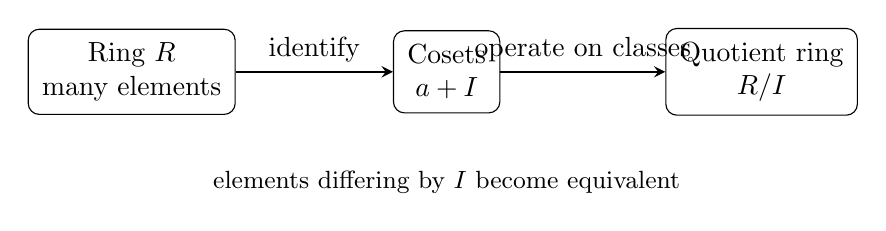
\begin{tikzpicture}[
    box/.style={draw,rounded corners,align=center,inner sep=5pt},
    >=stealth
]
\node[box] (R) at (0,0) {Ring \(R\)\\many elements};
\node[box] (classes) at (4,0) {Cosets\\\(a+I\)};
\node[box] (Q) at (8,0) {Quotient ring\\\(R/I\)};

\draw[->,thick] (R)--node[above]{identify}(classes);
\draw[->,thick] (classes)--node[above]{operate on classes}(Q);

\node at (4,-1.4) {\small elements differing by \(I\) become equivalent};
\end{tikzpicture}
\end{center}

%%%%%%%%%%%%%%%%%%%%%%%%%%%%%%%%%%%%%%%%%%%%%%%%%%%%%%%%%%%%
\subsection{Example: \(\Z/n\Z\)}
\label{subsec:ring-z-mod-n}
%%%%%%%%%%%%%%%%%%%%%%%%%%%%%%%%%%%%%%%%%%%%%%%%%%%%%%%%%%%%

The ideal

\[ n\Z \]

of \(\Z\) produces the quotient ring

\[ \Z/n\Z. \]

Its elements are

\[ [0]_n,[1]_n,\ldots,[n-1]_n. \]

Both addition and multiplication are performed modulo \(n\).

Thus modular arithmetic is simultaneously a quotient-group and quotient-ring
construction.

%%%%%%%%%%%%%%%%%%%%%%%%%%%%%%%%%%%%%%%%%%%%%%%%%%%%%%%%%%%%
\subsection{Worked Example: Arithmetic in a Quotient Ring}
\label{subsec:worked-quotient-ring}
%%%%%%%%%%%%%%%%%%%%%%%%%%%%%%%%%%%%%%%%%%%%%%%%%%%%%%%%%%%%

\begin{workedexamplebox}{Arithmetic in \(\Z/7\Z\)}

Compute

\[ [5]_7[6]_7+[4]_7. \]

\begin{tabularx}{\textwidth}{@{}>{\raggedright\arraybackslash}p{0.42\textwidth}X@{}}
Multiply representatives. & \(5\cdot6=30\)\\
Reduce modulo \(7\). & \([30]_7=[2]_7\)\\
Add \([4]_7\). & \([2]_7+[4]_7=[6]_7\)
\end{tabularx}

\begin{answerbox}
\[ [5]_7[6]_7+[4]_7=[6]_7. \]
\end{answerbox}
\end{workedexamplebox}

%%%%%%%%%%%%%%%%%%%%%%%%%%%%%%%%%%%%%%%%%%%%%%%%%%%%%%%%%%%%
\subsection{Ring Homomorphisms}
\label{subsec:ring-homomorphisms}
%%%%%%%%%%%%%%%%%%%%%%%%%%%%%%%%%%%%%%%%%%%%%%%%%%%%%%%%%%%%

\begin{definitionbox}{Ring Homomorphism}
A function
\[ \varphi:R\to S \]
between rings is a \emph{ring homomorphism} if
\[ \varphi(a+b)=\varphi(a)+\varphi(b) \]
and
\[ \varphi(ab)=\varphi(a)\varphi(b) \]
for all \(a,b\in R\).

Under the unital convention used here, we additionally require
\[ \varphi(1_R)=1_S. \]
\end{definitionbox}

A ring homomorphism preserves both algebraic operations.

%%%%%%%%%%%%%%%%%%%%%%%%%%%%%%%%%%%%%%%%%%%%%%%%%%%%%%%%%%%%
\subsection{Visualizing a Ring Homomorphism}
\label{subsec:visual-ring-homomorphism}
%%%%%%%%%%%%%%%%%%%%%%%%%%%%%%%%%%%%%%%%%%%%%%%%%%%%%%%%%%%%

\[
\begin{tikzcd}
R\times R \arrow[r,"+"] \arrow[d,"\varphi\times\varphi"'] &
R \arrow[d,"\varphi"]\\
S\times S \arrow[r,"+"] &
S
\end{tikzcd}
\qquad
\begin{tikzcd}
R\times R \arrow[r,"\cdot"] \arrow[d,"\varphi\times\varphi"'] &
R \arrow[d,"\varphi"]\\
S\times S \arrow[r,"\cdot"] &
S
\end{tikzcd}
\]

Both diagrams commute.

Thus \(\varphi\) preserves addition and multiplication.

%%%%%%%%%%%%%%%%%%%%%%%%%%%%%%%%%%%%%%%%%%%%%%%%%%%%%%%%%%%%
\subsection{Kernel of a Ring Homomorphism}
\label{subsec:ring-kernel}
%%%%%%%%%%%%%%%%%%%%%%%%%%%%%%%%%%%%%%%%%%%%%%%%%%%%%%%%%%%%

\begin{definitionbox}{Kernel of a Ring Homomorphism}
If
\[ \varphi:R\to S \]
is a ring homomorphism, then
\[ \Ker(\varphi)=\{r\in R:\varphi(r)=0_S\}. \]
\end{definitionbox}

The kernel is an ideal of \(R\).

This is the ring-theoretic analogue of kernels being normal subgroups in group
theory.

%%%%%%%%%%%%%%%%%%%%%%%%%%%%%%%%%%%%%%%%%%%%%%%%%%%%%%%%%%%%
\subsection{Image of a Ring Homomorphism}
\label{subsec:ring-image}
%%%%%%%%%%%%%%%%%%%%%%%%%%%%%%%%%%%%%%%%%%%%%%%%%%%%%%%%%%%%

The image is

\[ \Image(\varphi)=\{\varphi(r):r\in R\}. \]

The image forms a subring of the codomain.

%%%%%%%%%%%%%%%%%%%%%%%%%%%%%%%%%%%%%%%%%%%%%%%%%%%%%%%%%%%%
\subsection{Example: Reduction Modulo \(n\)}
\label{subsec:ring-reduction-homomorphism}
%%%%%%%%%%%%%%%%%%%%%%%%%%%%%%%%%%%%%%%%%%%%%%%%%%%%%%%%%%%%

Define

\[ \varphi:\Z\to\Z_n,\qquad\varphi(k)=[k]_n. \]

Then

\[ \varphi(a+b)=[a+b]_n=[a]_n+[b]_n \]

and

\[ \varphi(ab)=[ab]_n=[a]_n[b]_n. \]

Therefore \(\varphi\) is a ring homomorphism.

Its kernel is

\[ \Ker(\varphi)=n\Z. \]

Its image is all of \(\Z_n\).

%%%%%%%%%%%%%%%%%%%%%%%%%%%%%%%%%%%%%%%%%%%%%%%%%%%%%%%%%%%%
\subsection{First Isomorphism Theorem for Rings}
\label{subsec:first-isomorphism-ring}
%%%%%%%%%%%%%%%%%%%%%%%%%%%%%%%%%%%%%%%%%%%%%%%%%%%%%%%%%%%%

\begin{theorem}[First Isomorphism Theorem for Rings]
If
\[ \varphi:R\to S \]
is a ring homomorphism, then
\[ R/\Ker(\varphi)\cong\Image(\varphi). \]
\end{theorem}

This has exactly the same structural philosophy as the group-theoretic
version.

%%%%%%%%%%%%%%%%%%%%%%%%%%%%%%%%%%%%%%%%%%%%%%%%%%%%%%%%%%%%
\subsection{Visualizing the Ring Isomorphism Theorem}
\label{subsec:visual-ring-isomorphism}
%%%%%%%%%%%%%%%%%%%%%%%%%%%%%%%%%%%%%%%%%%%%%%%%%%%%%%%%%%%%

\begin{center}
\begin{tikzpicture}[
    node distance=16mm,
    box/.style={draw,rounded corners,align=center,inner sep=5pt},
    >=stealth
]
\node[box] (R) {\(R\)};
\node[box,right=of R] (Q) {\(R/\Ker(\varphi)\)};
\node[box,right=of Q] (I) {\(\Image(\varphi)\)};

\draw[->,thick] (R)--node[above]{collapse kernel}(Q);
\draw[->,thick] (Q)--node[above]{isomorphic}(I);
\end{tikzpicture}
\end{center}

The kernel records exactly which elements become indistinguishable under the
homomorphism.

%%%%%%%%%%%%%%%%%%%%%%%%%%%%%%%%%%%%%%%%%%%%%%%%%%%%%%%%%%%%
\subsection{Evaluation Homomorphisms}
\label{subsec:evaluation-homomorphisms}
%%%%%%%%%%%%%%%%%%%%%%%%%%%%%%%%%%%%%%%%%%%%%%%%%%%%%%%%%%%%

Let \(R\) be a commutative ring and choose \(a\in R\).

Define

\[ \operatorname{ev}_a:R[x]\to R \]

by

\[ \operatorname{ev}_a(f)=f(a). \]

The notation

\[ \operatorname{ev}_a \]

is read ``evaluation at \(a\).''

This is a ring homomorphism because

\[ (f+g)(a)=f(a)+g(a) \]

and

\[ (fg)(a)=f(a)g(a). \]

%%%%%%%%%%%%%%%%%%%%%%%%%%%%%%%%%%%%%%%%%%%%%%%%%%%%%%%%%%%%
\subsection{Kernel of Evaluation}
\label{subsec:kernel-evaluation}
%%%%%%%%%%%%%%%%%%%%%%%%%%%%%%%%%%%%%%%%%%%%%%%%%%%%%%%%%%%%

For

\[ \operatorname{ev}_a:R[x]\to R, \]

the kernel consists of polynomials satisfying

\[ f(a)=0. \]

When \(R\) is a field, the Factor Theorem gives

\[ f(a)=0\Longleftrightarrow (x-a)\mid f(x). \]

Therefore,

\[ \Ker(\operatorname{ev}_a)=(x-a). \]

This connects polynomial roots directly to ideals.

%%%%%%%%%%%%%%%%%%%%%%%%%%%%%%%%%%%%%%%%%%%%%%%%%%%%%%%%%%%%
\subsection{Characteristic of a Ring}
\label{subsec:ring-characteristic}
%%%%%%%%%%%%%%%%%%%%%%%%%%%%%%%%%%%%%%%%%%%%%%%%%%%%%%%%%%%%

Repeatedly add the multiplicative identity:

\[ 1,\qquad1+1,\qquad1+1+1,\qquad\ldots \]

Eventually this sum may become \(0\).

\begin{definitionbox}{Characteristic}
The \emph{characteristic} of a ring \(R\), written
\[ \operatorname{char}(R), \]
is the smallest positive integer \(n\) such that
\[ n\cdot1_R=0_R. \]

If no such positive integer exists, then
\[ \operatorname{char}(R)=0. \]
\end{definitionbox}

The notation

\[ \operatorname{char}(R) \]

is read ``the characteristic of \(R\).''

%%%%%%%%%%%%%%%%%%%%%%%%%%%%%%%%%%%%%%%%%%%%%%%%%%%%%%%%%%%%
\subsection{Examples of Characteristic}
\label{subsec:ring-characteristic-examples}
%%%%%%%%%%%%%%%%%%%%%%%%%%%%%%%%%%%%%%%%%%%%%%%%%%%%%%%%%%%%

For the integers,

\[ \operatorname{char}(\Z)=0. \]

Likewise,

\[ \operatorname{char}(\Q)=\operatorname{char}(\R)=\operatorname{char}(\C)=0. \]

For modular integers,

\[ \operatorname{char}(\Z_n)=n. \]

For example,

\[ \operatorname{char}(\Z_5)=5. \]

%%%%%%%%%%%%%%%%%%%%%%%%%%%%%%%%%%%%%%%%%%%%%%%%%%%%%%%%%%%%
\subsection{Characteristic of an Integral Domain}
\label{subsec:domain-characteristic}
%%%%%%%%%%%%%%%%%%%%%%%%%%%%%%%%%%%%%%%%%%%%%%%%%%%%%%%%%%%%

\begin{theorem}
The characteristic of an integral domain is either \(0\) or a prime number.
\end{theorem}

\begin{proof}
Suppose

\[ \operatorname{char}(R)=n>0. \]

Assume \(n\) is composite:

\[ n=ab \]

with

\[ 1<a<n,\qquad1<b<n. \]

Then

\[ (a\cdot1_R)(b\cdot1_R)=n\cdot1_R=0. \]

Since \(R\) has no zero divisors,

\[ a\cdot1_R=0 \]

or

\[ b\cdot1_R=0. \]

But this contradicts the minimality of \(n\).

Therefore \(n\) must be prime.
\end{proof}

%%%%%%%%%%%%%%%%%%%%%%%%%%%%%%%%%%%%%%%%%%%%%%%%%%%%%%%%%%%%
\subsection{Prime Ideals}
\label{subsec:prime-ideals}
%%%%%%%%%%%%%%%%%%%%%%%%%%%%%%%%%%%%%%%%%%%%%%%%%%%%%%%%%%%%

\begin{definitionbox}{Prime Ideal}
Let \(R\) be a commutative ring. A proper ideal \(P\subsetneq R\) is
\emph{prime} if
\[ ab\in P\Longrightarrow a\in P\text{ or }b\in P. \]
\end{definitionbox}

The symbol

\[ \subsetneq \]

means ``is a proper subset of.''

Thus

\[ P\subsetneq R \]

means \(P\subseteq R\) but \(P\neq R\).

%%%%%%%%%%%%%%%%%%%%%%%%%%%%%%%%%%%%%%%%%%%%%%%%%%%%%%%%%%%%
\subsection{Prime Ideals and Integral Domains}
\label{subsec:prime-ideal-domain}
%%%%%%%%%%%%%%%%%%%%%%%%%%%%%%%%%%%%%%%%%%%%%%%%%%%%%%%%%%%%

Prime ideals are closely connected with integral domains.

\begin{theorem}
For a commutative ring \(R\), an ideal \(P\) is prime if and only if
\[ R/P \]
is an integral domain.
\end{theorem}

This result turns a property of an ideal into a property of its quotient ring.

%%%%%%%%%%%%%%%%%%%%%%%%%%%%%%%%%%%%%%%%%%%%%%%%%%%%%%%%%%%%
\subsection{Maximal Ideals}
\label{subsec:maximal-ideals}
%%%%%%%%%%%%%%%%%%%%%%%%%%%%%%%%%%%%%%%%%%%%%%%%%%%%%%%%%%%%

\begin{definitionbox}{Maximal Ideal}
A proper ideal \(M\subsetneq R\) is \emph{maximal} if there is no ideal \(I\)
satisfying
\[ M\subsetneq I\subsetneq R. \]
\end{definitionbox}

Thus a maximal ideal is as large as a proper ideal can be.

%%%%%%%%%%%%%%%%%%%%%%%%%%%%%%%%%%%%%%%%%%%%%%%%%%%%%%%%%%%%
\subsection{Visualizing Maximality}
\label{subsec:visual-maximal-ideal}
%%%%%%%%%%%%%%%%%%%%%%%%%%%%%%%%%%%%%%%%%%%%%%%%%%%%%%%%%%%%

\begin{center}
\begin{tikzpicture}[>=stealth]
\node (M) at (0,0) {\(M\)};
\node (R) at (0,3) {\(R\)};

\draw[->,thick] (M)--(R);

\node[right=8mm] at (0,1.5) {no ideal strictly between};
\end{tikzpicture}
\end{center}

The diagram represents the inclusion relation

\[ M\subsetneq R \]

with no intermediate ideal.

%%%%%%%%%%%%%%%%%%%%%%%%%%%%%%%%%%%%%%%%%%%%%%%%%%%%%%%%%%%%
\subsection{Maximal Ideals and Fields}
\label{subsec:maximal-ideal-field}
%%%%%%%%%%%%%%%%%%%%%%%%%%%%%%%%%%%%%%%%%%%%%%%%%%%%%%%%%%%%

\begin{theorem}
Let \(R\) be a commutative ring with identity. A proper ideal \(M\) is maximal
if and only if
\[ R/M \]
is a field.
\end{theorem}

Compare this with the prime-ideal theorem:

\[
\begin{array}{c|c}
\text{Ideal property} & \text{Quotient property}\\
\hline
P\text{ prime} & R/P\text{ integral domain}\\
M\text{ maximal} & R/M\text{ field}
\end{array}
\]

%%%%%%%%%%%%%%%%%%%%%%%%%%%%%%%%%%%%%%%%%%%%%%%%%%%%%%%%%%%%
\subsection{Prime and Maximal Ideals in \(\Z\)}
\label{subsec:prime-maximal-z}
%%%%%%%%%%%%%%%%%%%%%%%%%%%%%%%%%%%%%%%%%%%%%%%%%%%%%%%%%%%%

Every ideal of \(\Z\) has the form

\[ (n). \]

If \(p\) is prime, then

\[ (p) \]

is both prime and maximal.

For example,

\[ \Z/(5)\cong\Z_5. \]

Since \(\Z_5\) is a field, \((5)\) is maximal.

%%%%%%%%%%%%%%%%%%%%%%%%%%%%%%%%%%%%%%%%%%%%%%%%%%%%%%%%%%%%
\subsection{Why Composite Moduli Produce Zero Divisors}
\label{subsec:composite-moduli-zero-divisors}
%%%%%%%%%%%%%%%%%%%%%%%%%%%%%%%%%%%%%%%%%%%%%%%%%%%%%%%%%%%%

Suppose

\[ n=ab \]

with

\[ 1<a<n,\qquad1<b<n. \]

Then in \(\Z_n\),

\[ [a]_n[b]_n=[ab]_n=[n]_n=[0]_n. \]

Neither factor is zero.

Therefore \(\Z_n\) has zero divisors whenever \(n\) is composite.

If \(p\) is prime, \(\Z_p\) is a field.

Thus

\begin{center}
\begin{tikzpicture}[
    node distance=15mm,
    box/.style={draw,rounded corners,align=center,inner sep=5pt},
    >=stealth
]
\node[box] (n) {\(\Z_n\)};
\node[box,below left=of n] (prime) {\(n=p\) prime};
\node[box,below right=of n] (comp) {\(n\) composite};
\node[box,below=of prime] (field) {field};
\node[box,below=of comp] (zero) {zero divisors};

\draw[->] (n)--(prime);
\draw[->] (n)--(comp);
\draw[->] (prime)--(field);
\draw[->] (comp)--(zero);
\end{tikzpicture}
\end{center}

%%%%%%%%%%%%%%%%%%%%%%%%%%%%%%%%%%%%%%%%%%%%%%%%%%%%%%%%%%%%
\subsection{Worked Example: Is \(\Z_8\) an Integral Domain?}
\label{subsec:worked-z8-domain}
%%%%%%%%%%%%%%%%%%%%%%%%%%%%%%%%%%%%%%%%%%%%%%%%%%%%%%%%%%%%

\begin{workedexamplebox}{Testing for an Integral Domain}

Determine whether \(\Z_8\) is an integral domain.

\begin{tabularx}{\textwidth}{@{}>{\raggedright\arraybackslash}p{0.42\textwidth}X@{}}
Look for nonzero zero divisors. & \([2]_8[4]_8=[8]_8\)\\
Reduce modulo \(8\). & \([8]_8=[0]_8\)\\
Check the factors. & \([2]_8\neq[0]_8,\quad[4]_8\neq[0]_8\)
\end{tabularx}

Thus \(\Z_8\) has zero divisors.

\begin{answerbox}
\(\Z_8\) is not an integral domain.
\end{answerbox}
\end{workedexamplebox}

%%%%%%%%%%%%%%%%%%%%%%%%%%%%%%%%%%%%%%%%%%%%%%%%%%%%%%%%%%%%
\subsection{Worked Example: Is \(\Z_7\) a Field?}
\label{subsec:worked-z7-field}
%%%%%%%%%%%%%%%%%%%%%%%%%%%%%%%%%%%%%%%%%%%%%%%%%%%%%%%%%%%%

\begin{workedexamplebox}{Testing a Modular Ring for a Field}

Determine whether \(\Z_7\) is a field.

\begin{tabularx}{\textwidth}{@{}>{\raggedright\arraybackslash}p{0.42\textwidth}X@{}}
Check the modulus. & \(7\text{ is prime}\)\\
Use the prime-modulus result. & Every nonzero class has an inverse.\\
Conclude. & \(\Z_7\text{ is a field.}\)
\end{tabularx}

For example,

\[ [3]_7[5]_7=[15]_7=[1]_7. \]

Thus

\[ [3]_7^{-1}=[5]_7. \]

\begin{answerbox}
\(\Z_7\) is a field.
\end{answerbox}
\end{workedexamplebox}

%%%%%%%%%%%%%%%%%%%%%%%%%%%%%%%%%%%%%%%%%%%%%%%%%%%%%%%%%%%%
\subsection{Ideals Generated by Several Elements}
\label{subsec:multiple-generated-ideals}
%%%%%%%%%%%%%%%%%%%%%%%%%%%%%%%%%%%%%%%%%%%%%%%%%%%%%%%%%%%%

For elements \(a_1,\ldots,a_n\in R\), the ideal they generate is written

\[ (a_1,\ldots,a_n). \]

In a commutative ring,

\[ (a_1,\ldots,a_n)=\{r_1a_1+\cdots+r_na_n:r_i\in R\}. \]

For example, in \(\Z\),

\[ (6,10)=(2). \]

The ideal generated by \(6\) and \(10\) is the same as the ideal generated by
their greatest common divisor.

%%%%%%%%%%%%%%%%%%%%%%%%%%%%%%%%%%%%%%%%%%%%%%%%%%%%%%%%%%%%
\subsection{Principal Ideal Domains}
\label{subsec:principal-ideal-domains}
%%%%%%%%%%%%%%%%%%%%%%%%%%%%%%%%%%%%%%%%%%%%%%%%%%%%%%%%%%%%

\begin{definitionbox}{Principal Ideal Domain}
A \emph{principal ideal domain}, abbreviated \emph{PID}, is an integral
domain in which every ideal is principal.
\end{definitionbox}

The abbreviation

\[ \mathrm{PID} \]

is read ``P-I-D'' or ``principal ideal domain.''

The integers \(\Z\) are a PID.

If \(F\) is a field, then

\[ F[x] \]

is also a PID.

%%%%%%%%%%%%%%%%%%%%%%%%%%%%%%%%%%%%%%%%%%%%%%%%%%%%%%%%%%%%
\subsection{Unique Factorization Domains}
\label{subsec:unique-factorization-domains}
%%%%%%%%%%%%%%%%%%%%%%%%%%%%%%%%%%%%%%%%%%%%%%%%%%%%%%%%%%%%

\begin{definitionbox}{Unique Factorization Domain}
A \emph{unique factorization domain}, abbreviated \emph{UFD}, is an integral
domain in which every nonzero nonunit can be factored into irreducible
elements, uniquely up to multiplication by units and rearrangement.
\end{definitionbox}

The abbreviation

\[ \mathrm{UFD} \]

is read ``U-F-D.''

The integers are a familiar example.

%%%%%%%%%%%%%%%%%%%%%%%%%%%%%%%%%%%%%%%%%%%%%%%%%%%%%%%%%%%%
\subsection{Euclidean Domains}
\label{subsec:euclidean-domains}
%%%%%%%%%%%%%%%%%%%%%%%%%%%%%%%%%%%%%%%%%%%%%%%%%%%%%%%%%%%%

A Euclidean domain is an integral domain equipped with a division algorithm
controlled by a suitable size function.

Examples include

\[ \Z \]

and

\[ F[x] \]

when \(F\) is a field.

Euclidean domains allow versions of the Euclidean algorithm used for greatest
common divisors.

%%%%%%%%%%%%%%%%%%%%%%%%%%%%%%%%%%%%%%%%%%%%%%%%%%%%%%%%%%%%
\subsection{Hierarchy of Important Domains}
\label{subsec:domain-hierarchy}
%%%%%%%%%%%%%%%%%%%%%%%%%%%%%%%%%%%%%%%%%%%%%%%%%%%%%%%%%%%%

A major hierarchy in commutative algebra is

\begin{center}
\begin{tikzpicture}[
    node distance=10mm,
    box/.style={draw,rounded corners,align=center,inner sep=5pt,font=\small},
    >=stealth
]
\node[box] (field) {Field};
\node[box,below=of field] (ed) {Euclidean domain};
\node[box,below=of ed] (pid) {Principal ideal domain};
\node[box,below=of pid] (ufd) {Unique factorization domain};
\node[box,below=of ufd] (id) {Integral domain};

\draw[->] (field)--(ed);
\draw[->] (ed)--(pid);
\draw[->] (pid)--(ufd);
\draw[->] (ufd)--(id);
\end{tikzpicture}
\end{center}

Every field is a Euclidean domain, every Euclidean domain is a PID, every PID
is a UFD, and every UFD is an integral domain.

The converses are generally false.

These ideas are developed more deeply in
\cref{sec:commutative-algebra}.

%%%%%%%%%%%%%%%%%%%%%%%%%%%%%%%%%%%%%%%%%%%%%%%%%%%%%%%%%%%%
\subsection{Irreducible Elements}
\label{subsec:irreducible-elements}
%%%%%%%%%%%%%%%%%%%%%%%%%%%%%%%%%%%%%%%%%%%%%%%%%%%%%%%%%%%%

\begin{definitionbox}{Irreducible Element}
A nonzero nonunit \(p\in R\) is \emph{irreducible} if
\[ p=ab \]
implies that \(a\) or \(b\) is a unit.
\end{definitionbox}

Irreducible elements generalize prime numbers as objects that cannot be
factored nontrivially.

%%%%%%%%%%%%%%%%%%%%%%%%%%%%%%%%%%%%%%%%%%%%%%%%%%%%%%%%%%%%
\subsection{Prime Elements}
\label{subsec:prime-elements}
%%%%%%%%%%%%%%%%%%%%%%%%%%%%%%%%%%%%%%%%%%%%%%%%%%%%%%%%%%%%

\begin{definitionbox}{Prime Element}
A nonzero nonunit \(p\) in an integral domain is \emph{prime} if
\[ p\mid ab\Longrightarrow p\mid a\text{ or }p\mid b. \]
\end{definitionbox}

Every prime element is irreducible.

The converse does not hold in every integral domain.

In a UFD, irreducible and prime elements coincide.

%%%%%%%%%%%%%%%%%%%%%%%%%%%%%%%%%%%%%%%%%%%%%%%%%%%%%%%%%%%%
\subsection{Rings of Functions}
\label{subsec:rings-of-functions}
%%%%%%%%%%%%%%%%%%%%%%%%%%%%%%%%%%%%%%%%%%%%%%%%%%%%%%%%%%%%

Let \(X\) be a set.

Consider real-valued functions

\[ f:X\to\R. \]

Define addition and multiplication pointwise:

\[ (f+g)(x)=f(x)+g(x), \]

\[ (fg)(x)=f(x)g(x). \]

These functions form a commutative ring.

The zero element is the zero function

\[ 0(x)=0, \]

and the multiplicative identity is the constant function

\[ 1(x)=1. \]

%%%%%%%%%%%%%%%%%%%%%%%%%%%%%%%%%%%%%%%%%%%%%%%%%%%%%%%%%%%%
\subsection{Rings as a Common Language}
\label{subsec:rings-common-language}
%%%%%%%%%%%%%%%%%%%%%%%%%%%%%%%%%%%%%%%%%%%%%%%%%%%%%%%%%%%%

Ring theory unifies many mathematical objects.

\[
\begin{array}{c|c|c}
\text{Ring} & \text{Elements} & \text{Operations}\\
\hline
\Z & \text{integers} & +,\cdot\\
\Z_n & \text{residue classes} & +,\cdot\pmod n\\
R[x] & \text{polynomials} & +,\cdot\\
M_n(R) & \text{matrices} & +,\cdot\\
R^X & \text{functions }X\to R & \text{pointwise }+,\cdot
\end{array}
\]

The elements look very different, but the same structural ideas apply.

%%%%%%%%%%%%%%%%%%%%%%%%%%%%%%%%%%%%%%%%%%%%%%%%%%%%%%%%%%%%
\subsection{A Structural Map of Ring Theory}
\label{subsec:ring-theory-map}
%%%%%%%%%%%%%%%%%%%%%%%%%%%%%%%%%%%%%%%%%%%%%%%%%%%%%%%%%%%%

\begin{center}
\begin{tikzpicture}[
    node distance=10mm and 14mm,
    box/.style={draw,rounded corners,align=center,inner sep=4pt,font=\small},
    >=stealth
]
\node[box] (ring) {Ring};
\node[box,below left=of ring] (elements) {Special elements};
\node[box,below right=of ring] (sub) {Substructures};

\node[box,below left=of elements] (units) {Units};
\node[box,below=of elements] (zero) {Zero divisors};
\node[box,below right=of elements] (nil) {Nilpotents};

\node[box,below left=of sub] (subring) {Subrings};
\node[box,below right=of sub] (ideal) {Ideals};

\node[box,below=of ideal] (quot) {Quotient rings};
\node[box,below=of quot] (hom) {Homomorphisms};
\node[box,below=of hom] (iso) {Isomorphism theorems};

\draw[->] (ring)--(elements);
\draw[->] (ring)--(sub);
\draw[->] (elements)--(units);
\draw[->] (elements)--(zero);
\draw[->] (elements)--(nil);
\draw[->] (sub)--(subring);
\draw[->] (sub)--(ideal);
\draw[->] (ideal)--(quot);
\draw[->] (quot)--(hom);
\draw[->] (hom)--(iso);
\end{tikzpicture}
\end{center}

%%%%%%%%%%%%%%%%%%%%%%%%%%%%%%%%%%%%%%%%%%%%%%%%%%%%%%%%%%%%
\subsection{Common Errors in Ring Theory}
\label{subsec:common-ring-errors}
%%%%%%%%%%%%%%%%%%%%%%%%%%%%%%%%%%%%%%%%%%%%%%%%%%%%%%%%%%%%

\subsubsection{Assuming Multiplication Is Commutative}

In an arbitrary ring,

\[ ab\neq ba \]

may occur.

Matrix rings provide standard counterexamples.

%%%%%%%%%%%%%%%%%%%%%%%%%%%%%%%%%%%%%%%%%%%%%%%%%%%%%%%%%%%%
\subsubsection{Assuming Nonzero Elements Can Be Cancelled}

Cancellation may fail when zero divisors exist.

From

\[ ab=ac \]

one cannot conclude \(b=c\) in an arbitrary ring.

%%%%%%%%%%%%%%%%%%%%%%%%%%%%%%%%%%%%%%%%%%%%%%%%%%%%%%%%%%%%
\subsubsection{Assuming Every Nonzero Element Is a Unit}

That property characterizes division rings and fields, not arbitrary rings.

For example,

\[ 2\in\Z \]

is nonzero but not a unit.

%%%%%%%%%%%%%%%%%%%%%%%%%%%%%%%%%%%%%%%%%%%%%%%%%%%%%%%%%%%%
\subsubsection{Confusing a Subring with an Ideal}

A subring must itself form a ring.

An ideal must additionally absorb multiplication by arbitrary elements of the
larger ring.

Ideals are the correct objects for forming quotient rings.

%%%%%%%%%%%%%%%%%%%%%%%%%%%%%%%%%%%%%%%%%%%%%%%%%%%%%%%%%%%%
\subsubsection{Confusing Prime Elements and Prime Ideals}

A prime element is an element of a ring.

A prime ideal is a subset of a ring satisfying an ideal-theoretic property.

The concepts are related but not identical.

%%%%%%%%%%%%%%%%%%%%%%%%%%%%%%%%%%%%%%%%%%%%%%%%%%%%%%%%%%%%
\subsubsection{Assuming Irreducible Means Prime Everywhere}

In \(\Z\) the concepts agree.

In arbitrary integral domains, an irreducible element need not be prime.

%%%%%%%%%%%%%%%%%%%%%%%%%%%%%%%%%%%%%%%%%%%%%%%%%%%%%%%%%%%%
\subsubsection{Forgetting Ring Conventions}

Some authors require rings to have a multiplicative identity and some do not.

Some definitions of ring homomorphism require preservation of \(1\), while
others do not.

Always determine the convention being used.

%%%%%%%%%%%%%%%%%%%%%%%%%%%%%%%%%%%%%%%%%%%%%%%%%%%%%%%%%%%%
\subsection{Applications and Connections}
\label{subsec:ring-applications}
%%%%%%%%%%%%%%%%%%%%%%%%%%%%%%%%%%%%%%%%%%%%%%%%%%%%%%%%%%%%

\begin{applicationbox}
\textbf{Number Theory.}
The integers, modular arithmetic, algebraic integers, and congruences are
naturally studied through rings and ideals.

\medskip

\textbf{Polynomial Algebra.}
Polynomial rings provide the algebraic setting for factorization, roots, and
equations.

\medskip

\textbf{Linear Algebra.}
Matrices form noncommutative rings, and endomorphisms of vector spaces form
rings under addition and composition.

\medskip

\textbf{Geometry.}
Polynomial rings and quotient rings form the algebraic foundation of
algebraic geometry.

\medskip

\textbf{Commutative Algebra.}
Ideals, prime ideals, localization, modules, and factorization are developed
systematically from ring theory.

\medskip

\textbf{Field Theory.}
Fields are special commutative rings in which every nonzero element is
invertible.

\medskip

\textbf{Coding and Cryptography.}
Finite rings and polynomial quotient rings appear in coding theory,
cryptography, and computational algebra.
\end{applicationbox}

%%%%%%%%%%%%%%%%%%%%%%%%%%%%%%%%%%%%%%%%%%%%%%%%%%%%%%%%%%%%
\subsection{Exercises}
\label{subsec:ring-theory-exercises}
%%%%%%%%%%%%%%%%%%%%%%%%%%%%%%%%%%%%%%%%%%%%%%%%%%%%%%%%%%%%

\begin{exercise}[1]
Verify that \(\Z\) is a commutative ring.
\end{exercise}

\begin{exercise}[1]
Explain why \(M_2(\R)\) is generally noncommutative.
\end{exercise}

\begin{exercise}[1]
Determine whether \(\Z_6\) contains zero divisors.
\end{exercise}

\begin{exercise}[1]
Find all zero divisors in \(\Z_8\).
\end{exercise}

\begin{exercise}[1]
Find all units in \(\Z_8\).
\end{exercise}

\begin{exercise}[2]
Find all units in \(\Z_{12}\).
\end{exercise}

\begin{exercise}[2]
Find all idempotent elements in \(\Z_6\).
\end{exercise}

\begin{exercise}[2]
Find all nilpotent elements in \(\Z_8\).
\end{exercise}

\begin{exercise}[2]
Prove that
\[ a0=0a=0 \]
in every ring.
\end{exercise}

\begin{exercise}[2]
Prove
\[ (-a)b=-(ab). \]
\end{exercise}

\begin{exercise}[2]
Prove
\[ (-a)(-b)=ab. \]
\end{exercise}

\begin{exercise}[2]
Expand
\[ (a+b)^3 \]
without assuming multiplication is commutative.
\end{exercise}

\begin{exercise}[2]
Explain exactly where commutativity is needed to simplify the result to the
usual binomial formula.
\end{exercise}

\begin{exercise}[1]
Determine whether \(\Z_{10}\) is an integral domain.
\end{exercise}

\begin{exercise}[1]
Determine whether \(\Z_{11}\) is an integral domain.
\end{exercise}

\begin{exercise}[1]
Determine whether \(\Z_{11}\) is a field.
\end{exercise}

\begin{exercise}[2]
Prove that if \(n\) is composite, then \(\Z_n\) has zero divisors.
\end{exercise}

\begin{exercise}[2]
Show that the nonzero elements of a field form an abelian group under
multiplication.
\end{exercise}

\begin{exercise}[2]
Use the subring test to show that
\[ \Z\subseteq\Q \]
is a subring.
\end{exercise}

\begin{exercise}[2]
Show that
\[ 2\Z \]
is an ideal of \(\Z\).
\end{exercise}

\begin{exercise}[2]
Show that
\[ 3\Z \]
is an ideal of \(\Z\).
\end{exercise}

\begin{exercise}[2]
Determine
\[ (6)+(15) \]
as an ideal of \(\Z\).
\end{exercise}

\begin{exercise}[2]
Determine
\[ (6)\cap(15) \]
in \(\Z\).
\end{exercise}

\begin{exercise}[2]
Describe the quotient ring
\[ \Z/4\Z. \]
\end{exercise}

\begin{exercise}[2]
Construct the addition and multiplication tables for \(\Z_4\).
\end{exercise}

\begin{exercise}[2]
Using the multiplication table, identify the units and zero divisors of
\(\Z_4\).
\end{exercise}

\begin{exercise}[2]
Let
\[ \varphi:\Z\to\Z_5,\qquad\varphi(n)=[n]_5. \]
Find its kernel and image.
\end{exercise}

\begin{exercise}[3]
Use the First Isomorphism Theorem to prove
\[ \Z/5\Z\cong\Z_5. \]
\end{exercise}

\begin{exercise}[2]
Let
\[ \operatorname{ev}_2:\R[x]\to\R \]
be evaluation at \(2\). Find
\[ \operatorname{ev}_2(x^3-4x+1). \]
\end{exercise}

\begin{exercise}[2]
Determine the kernel of
\[ \operatorname{ev}_2:\R[x]\to\R. \]
\end{exercise}

\begin{exercise}[2]
Find
\[ \operatorname{char}(\Z_{12}). \]
\end{exercise}

\begin{exercise}[2]
Find the characteristics of
\[ \Z,\qquad\Q,\qquad\R,\qquad\Z_7. \]
\end{exercise}

\begin{exercise}[3]
Prove that the characteristic of an integral domain is either \(0\) or prime.
\end{exercise}

\begin{exercise}[2]
Determine whether the ideal
\[ (5)\subseteq\Z \]
is prime.
\end{exercise}

\begin{exercise}[2]
Determine whether
\[ (6)\subseteq\Z \]
is prime.
\end{exercise}

\begin{exercise}[2]
Determine whether
\[ (7)\subseteq\Z \]
is maximal.
\end{exercise}

\begin{exercise}[2]
Explain why
\[ \Z/(7) \]
is a field.
\end{exercise}

\begin{exercise}[2]
Explain why
\[ \Z/(8) \]
is not a field.
\end{exercise}

\begin{exercise}[2]
Let
\[ f(x)=2x+1,\qquad g(x)=3x+1 \]
in \(\Z_6[x]\). Compute \(f(x)g(x)\) and compare the degrees.
\end{exercise}

\begin{exercise}[2]
Show that the real-valued functions on a set \(X\) form a commutative ring
under pointwise operations.
\end{exercise}

\begin{exercise}[3]
Show that the units of a ring form a group under multiplication.
\end{exercise}

\begin{exercise}[3]
Prove that every field is an integral domain.
\end{exercise}

\begin{exercise}[3]
Give an example of an integral domain that is not a field.
\end{exercise}

\begin{exercise}[3]
Give an example of a ring that is not an integral domain.
\end{exercise}

\begin{exercise}[3]
Explain the structural analogy among
\[ \text{normal subgroups},\qquad\text{ideals},\qquad\text{kernels}. \]
\end{exercise}

%%%%%%%%%%%%%%%%%%%%%%%%%%%%%%%%%%%%%%%%%%%%%%%%%%%%%%%%%%%%
\subsection{Section Connections}
\label{subsec:ring-theory-connections}
%%%%%%%%%%%%%%%%%%%%%%%%%%%%%%%%%%%%%%%%%%%%%%%%%%%%%%%%%%%%

\chapterconnection{
Ring theory provides the canonical foundation for algebraic systems with two
compatible operations. Field theory strengthens ring structure by requiring
multiplicative inverses for every nonzero element. Galois theory studies field
extensions and their symmetry groups. Module theory replaces vector spaces'
field scalars with ring scalars. Commutative algebra later develops ideals,
prime spectra, localization, Noetherian conditions, and factorization much
more deeply. Noncommutative algebra studies rings in which multiplication
cannot be reordered. Algebraic geometry, algebraic number theory,
representation theory, and homological algebra all depend heavily on the ring
structures introduced here.
}

%%%%%%%%%%%%%%%%%%%%%%%%%%%%%%%%%%%%%%%%%%%%%%%%%%%%%%%%%%%%
% SECTION SOURCE TRACKING
%%%%%%%%%%%%%%%%%%%%%%%%%%%%%%%%%%%%%%%%%%%%%%%%%%%%%%%%%%%%

%------------------------------------------------------------
% 1.5 Ring Theory
%------------------------------------------------------------
%
% Sources:
%   - Thomas W. Judson, Abstract Algebra: Theory and Applications.
%     Key: judson2025abstractalgebra
%
% Used for:
%   - ring definitions and basic identities;
%   - integral domains and fields;
%   - units and zero divisors;
%   - polynomial rings;
%   - ideals and quotient rings;
%   - ring homomorphisms, kernels, and images;
%   - characteristic;
%   - prime and maximal ideals;
%   - factorization terminology and standard examples.
%
% Notes:
%   - Ring theory is the canonical location for the fundamental definitions
%     and elementary structural results concerning rings.
%   - Detailed field theory is deferred to Section 1.6.
%   - Detailed module theory is deferred to Section 1.8.
%   - Advanced ideal theory, localization, Noetherian rings, dimension, and
%     related topics are deferred to Section 1.9 Commutative Algebra.
%   - Deeper noncommutative phenomena are deferred to Section 1.10.
%   - Visualizations and exposition are independently developed for this text.
%
\nocite{judson2025abstractalgebra}